\documentclass[a4paper,11pt]{article}
%OFFICIAL:
\usepackage[top=1.18in, bottom=1.18in, left=1.18in, right=0.98in, a4paper]{geometry}
%SMALLER
% \usepackage[top=0.98in, bottom=0.98in, left=0.98in, right=0.7in, a4paper]{geometry}
% \usepackage{fontspec}
% \setmainfont{Liberation Sans}

\renewcommand{\baselinestretch}{1} 
\usepackage{wrapfig}

\usepackage{import}
\usepackage{ifthen}
\usepackage{eurosym}
\usepackage{wrapfig}
\usepackage{arydshln}
\usepackage[utf8]{inputenc}
\usepackage{url}

%opening
\title{Competitive Lazy Grounding for Answer Set Programming}
\author{Bart Bogaerts, Francesco Ricca, Antonius Weinzierl}

\input{idp-latex/idp-latex}
\usepackage{svg}
\usepackage{tikz}
\usetikzlibrary{positioning}
\usetikzlibrary{graphs, graphs.standard, quotes}% quotes library is for the [""] edges

\tikzset{main node/.style={circle,fill=yellow!20,draw,minimum size=1.42cm,inner sep=0pt},
            }

\usepackage{graphicx}
\newcommand{\alphasolver}{\logicname{alpha}}
\newcommand{\Omiga}{\logicname{Omiga}}
\newcommand{\GASP}{\logicname{GASP}}
\newcommand{\ASPeRiX}{\logicname{ASPeRiX}}
\newcommand{\GalliWasp}{\logicname{GalliWasp}}
% \newcommand{}{\logicname{}}
\newcommand{\wasp}{\logicname{wasp}}

\usepackage{paralist}
\renewenvironment{thebibliography}[1]{%
%   \section*{\refname}%
  \let\par\relax\let\newblock\relax%
%   \inparaenum[{[}1{]}]}{\endinparaenum}
  \compactenum[{[}1{]}]}{\endcompactenum}
% \renewcommand{\bibitem}[1]{\item}

\newcommand\fwohelp[1]{\textit{#1}


}
\declaretheoremstyle[
    headfont=\bfseries, 
    notebraces={}{ },
    notefont=\bfseries\itshape,
    headformat={\NAME\ \NUMBER.\NOTE},
%     bodyfont=\normalfont\itshape,
    bodyfont=\normalfont,
    headpunct={},
%     postheadspace=\newline,
%     postheadhook={\textcolor{red}{\rule[.6ex]{\linewidth}{0.4pt}}\\},
    spacebelow=\parsep,
    spaceabove=\parsep,
%     mdframed={
%         backgroundcolor=red!20, 
%             linecolor=red!30, 
%             innertopmargin=6pt,
%             roundcorner=5pt, 
%             innerbottommargin=6pt, 
%             skipabove=\parsep, 
%             skipbelow=\parsep } 
]{WPStyle}

\declaretheorem[style=WPStyle,	qed=$\blacktriangle$, name=Work Package]{WP}
\declaretheorem[style=WPStyle,	qed=$\blacktriangle$, name=Objective ]{OBJ}
\newcommand\WPref[1]{\textbf{WP\ref{#1}}}
\newcommand\OBJref[1]{\textbf{OBJ\ref{#1}}}
\newcommand\CATref[1]{\textbf{(\ref{#1})}}
\newcommand{\pk}[1]{{\color{green}#1}}
\setdefaultenum{\bfseries(i)}{}{}{}
\def\mapf{{\bf MAPF}\xspace}
% \setlength{\textfloatsep}{100pt plus 10.0pt minus 2.0pt}
% \setlength{\floatsep}{100pt plus 10.0pt minus 2.0pt}
\usepackage[many]{tcolorbox}
\newtcolorbox{framefloat}[1][!tb]{arc=10pt,outer arc=2pt,boxrule=1pt,
  colframe=black,colback=white,float=#1,boxsep=-1mm,enlarge top by=-2mm,enlarge bottom by=-2mm}
  
% \setlength\intextsep{2\baselineskip plus 0.2\baselineskip minus 0.2\baselineskip}


% \renewenvironment{thebibliography}[1]{\let\par\relax%
%   \section*{\refname}\inparaenum[\mybullet]}{\endinparaenum}
% \let\oldbibitem\bibitem
% \renewcommand{\bibitem}{\item \oldbibitem}

% \renewenvironment{thebibliography}[1]{%
% %        \section*{\refname}
%        \let\par\relax\let\newblock\relax
%        \inparaenum
%        \let\olditem\item
%        \renewcommand{\item}[1][]{\textbf\olditem}
%      }{\endinparaenum}

\begin{document}
\setdefaultleftmargin{1em}{0.8em}{0.5em}{1.7em}{1em}{1em}  
% \maketitle


\todo{Drop FCG}

\todo{Drop disj Just} 

\todo{Split ``transition systems'' (for studying propagation power) and ``proof theory'' (for size of the constructed proof)}

\todo{Wasp vs clasp?}
% \begin{abstract}
% 
% \end{abstract}
% \todo{Rollen Wenen calabria verkleinen}
% \todo{verzwak ook statement ``werken samen met'' -> zeg iets als ``similar running projects''}
% \todo{check consumable budget}

\section{Rationale and Positioning with Regard to State of the Art}
% \todo{CHECK \url{https://www.cambridge.org/core/services/aop-cambridge-core/content/view/4ACBFA9C729F45DDC90942758BFFCACA/S1471068410700254a.pdf/constraints_lazy_constraints_or_propagators_in_asp_solving_an_empirical_analysis.pdf} \cite{tplp/CuteriDRS17}}
Answer Set Programming (ASP) is well-established as a knowledge representation paradigm. ASP stems from the idea that stable model semantics of logic problems can be utilized to encode search problems. It is especially useful for encoding NP-complete problems and this property is recently exploited in application domains such as machine learning, robotics, data-integration, biology, planning, phylogenetic inference and product configuration. ASP has a rich first-order language ASP-Core2 to effectively represent knowledge in the mentioned domains and has efficient solvers built on top of conflict-driven clause learning (CDCL) from satisfiability solving and lazy clause generation.

\begin{framefloat}[h]
Traditional ASP systems work in two phases: \textbf{grounding} and \textbf{solving}. This works well for problems where the grounding is not too large.
\end{framefloat}

Programs written in ASP-Core2 language has  first-order variables in them and these need to be eliminated to feed the program into an ASP solver. This process is called grounding. To this day, most of the effort on ASP focused on improving the efficiency of ASP solvers while the grounding methods changed very little. Recently, though, the community started showing interest in better grounding methods since there are interesting problems where grounding is the bottleneck \cite{lpnmr/BalducciniLS13}. Examples to such problems include planning with a potentially large number of time-steps; queries such as reachability on large graphs; and problems that have a lot of unnecessary information when fully grounded but are simple in nature. There are already ongoing efforts to address this grounding bottleneck. Intelligent grounding \cite{ia/CalimeriFPZ17} and rule decomposition \cite{lopstr/BichlerMW16} aim to reduce the size of grounding where possible. For query problems, top-down evaluation utilizing \emph{magic sets} \cite{pods/BancilhonMSU86,ai/AlvianoFGL12} is used. For planning problems, \emph{incremental grounding} \cite{aicom/GebserSS11} is used to ground the next time steps only if a solution does not exist for the current number of time-steps. This general idea of grounding only as much as needed is called lazy grounding. Bottom-up lazy grounding systems include \Omiga \mycite{omiga}, \GASP \mycite{gasp}, \ASPeRiX \mycite{asperix} and the recently introduced \alphasolver \mycite{alpha} that integrates lazy grounding with a CDCL solver. Also top-down lazy grounding techniques (for a language related to ASP) \mycite{lazyGrounding} and top-down stable model generation techniques that avoid grounding  \cite{lopstr/MarpleG12,corr/MarpleSG17} exist.

\begin{framefloat}[ht]
Lazy grounding systems interleave the two phases, with as aim to \textbf{only ground those parts} that are \textbf{relevant} for the solver, to overcome the \textbf{grounding bottleneck}.
\end{framefloat}

While these lazy grounding methods outperform the usual ground-and-solve approaches on problems where grounding is the bottleneck, they are far from competitive on standard ASP problems \cite{jair/GebserMR17}. This is not surprising since lazy grounding is tailored for the former kind of problems, but currently we do not have an understanding of where the disparity in performance on the latter comes from. One reason may be that ground-and-solve approaches are more matured since they have been being optimized for years by now, but some part of the performance difference should be caused by differences in algorithms, such as missed propagation due to not constructing parts of the grounding. In this project, we investigate all the factors that determine the differences in speed between these systems. Based on that analysis, we develop new lazy grounding techniques and systems that circumvent the greatest bottlenecks. Our hypothesis is that these improvements will prove valuable both in traditional applications and on applications where lazy grounding systems are superior to ground-and-solve systems.




The focus of this project is on lazy grounding with a CDCL solver as backend, since 
CDCL has been responsible for one of the greatest performance boosts in SAT- and ASP-solving. 
% It has proven very valuable in many applications, and 
We believe CDCL to be a strong foundation to build search algorithms on. 
% Existing lazy grounding systems not based on CDCL often suffer from poor search performance. 
In particular, the basis of this project will be \alphasolver, the only CDCL-based lazy grounding algorithm for ASP. 
% Recently \cite{\refto{LazyGrounding}} introduced lazy model expansion for IDP, which is in spirit very similar to ASP. 
% The methods developed there were conjectured to also be applicable to ASP, but this hypothesis has not been tested yet.
% A big difference between lazy model expansion and the \alphasolver algorithm is that lazy model expansion works goal-directed (top-down through the underlying logic program) and exploits properties of the well-founded semantics, while \alphasolver works bottom-up and exploits properties of the stable semantics to avoid grounding too much. 
In this project, we investigate to which extent it is possible to integrate top-down (goal-directed) lazy grounding techniques (such as \cite{corr/MarpleSG17} and those developed for the IDP system \cite{\refto{LazyGrounding}}) in \alphasolver and more generally, extend the \alphasolver algorithm with techniques that compensate for its weaknesses, while preserving its strengths. In pilot research for the current project, we took a first, promising, step in this direction  by using a justification-based top-down analysis whenever \alphasolver arrives in a conflict it cannot easily resolve \cite{ijcai/BogaertsW18}. %\todo{Bovenstaande paragraaf is een beetje warrig. Wat komt broes hier ineens doen?}

\begin{framefloat}[ht]
On traditional applications, lazy grounding systems are often orders of magnitude slower than ground-and-solve systems. 
We research \textbf{why} there is such a big performance gap and develop \textbf{novel lazy grounding algorithms} that do not suffer from this. 
\end{framefloat}

We ground our research by testing it on ASP models for Multi Agent Path Finding (\mapf), which can be modeled as a planning problem or a graph problem \cite{tajelipirbazari2022multi}. \mapf is both hard and related to real world applications such as automated warehouses. Also, it has variants which are practically harder to solve (and at least as hard theoretically) [REFER TO THESIS], which will allow for testing our approach on incrementally harder versions of the same fundamental problem.

The outcome of this project is manifold. 
First of all, there will be an increased understanding of how different techniques to avoid grounding relate.
Second, there will be a clear overview of which factors influence the performance differences between lazy grounding systems and traditional ground-and-solve systems. 
Third, we develop novel lazy grounding techniques that combine elements of top-down and bottom-up reasoning.
Fourth, we ground and evaluate our research on \mapf using ASP. 

\section{Scientific Research Objectives}


We categorize our objectives as follows: \begin{inparaenum}
\item \label{cat:study} deeply understanding the literature on lazy grounding and analyzing them 
\item \label{cat:dev} developing novel algorithms for lazy grounding, 
\item \label{cat:app} applying and evaluating said algorithms.
\end{inparaenum}
 To achieve \CATref{cat:study}, we elaborate our objectives as follows:
 
 \begin{OBJ} \label{obj:literature} Develop a clear understanding of existing lazy grounding algorithms for ASP and their relationships with each other, and the cases where they are best used.
 \end{OBJ}
\begin{OBJ} \label{obj:factors} Identify the factors that make the existing algorithms perform poorly, and quantify the effects of these factors.
 \end{OBJ}
To develop novel algorithms for lazy grounding \CATref{cat:dev}, we believe a good starting point would be to combine bottom-up and top-down reasoning approaches. Also, we can increment on existing algorithms in consideration of their current shortcomings. 
\begin{OBJ} \label{obj:extend} Extend the current algorithms by addressing the most important factors identified in \OBJref{obj:factors}.
 \end{OBJ}
\begin{OBJ} \label{obj:dev} Develop lazy grounding algorithms that combine top-down and bottom-up reasoning approaches
 \end{OBJ}
We propose concrete ways to achieve \OBJref{obj:extend} and \OBJref{obj:dev} objectives in our work packages.
We would like to evaluate \CATref{cat:app} our novel algorithms by applying them to challenging problems and existing lazy grounding benchmarks.
\begin{OBJ} \label{evaluate} Evaluate our novel algorithms on \mapf and existing benchmarks for lazy grounding.
 \end{OBJ}



\begin{framefloat}[h]
The result of this project is a \textbf{clear analysis of the strengths and weaknesses} of existing lazy grounding techniques and \textbf{novel algorithms that overcome those weaknesses}. As a result, answer set programming will be applicable to a \textbf{broad class of problems} that are currently unsolvable due to the grounding bottleneck.
\end{framefloat}


 
%  \begin{OBJ}
%  \end{OBJ}

\section{Research Methodology and Work Plan}
% \todo{KERSTEN:Pag. 6: na je methodology van WP 1 tot 12 viel het me op dat je weinig vermeld over wat de taak/support is van Vienna/Calabria binnen deze WPs? Vooral omdat je onder punt 4 wel organisatie vermeld en daar de partnerships aanhaalt. Verder, hier begin je ook ineens over PhD 1 en 2 (dit wordt duidelijk bij 6. Budget), misschien kan je hier ook kort uitleggen dat het project steunt op 2 studenten ter voorbereiding van PhD en misschien ook hoe je deze werkverdeling ziet? Vooral omdat ik de WP 1-12 lees als geheel en dan ineens merk dat dit verdeeld wordt over 2 personen?
% }
% \todo{Say something about benchmarks. That all of work packages X-Y contain a validation component. Say on what we test them. }
To analyze the existing algorithms, we study the existing literature and test them on \mapf. This way, we can pinpoint the shortcomings of these algorithms on a relevant and practical problem.


For implementing both our novel algorithms and existing algorithms in the literature, we use the recently developed and promising ASP solver WASP \mycite{wasp}. WASP is a state-of-the-art solver with useful features focusing on extendibility. This means we can more easily modify the inner workings of the solver compared to other solvers, which will prove useful as we describe in our work packages. We believe using an existing and well-engineered solver like WASP will save us precious time from implementing our own. WASP is developed in University of Calabria and we plan a research visit there to utilize their expertise. Our strategy will be to implement our lazy grounding algorithms as custom theory propagators, which can be efficiently done using WASP \mycite{wasp}.
For experimental analysis, we reimplement \alphasolver  on WASP in a modular way such that we can enable or disable different parts of the algorithm. This would allow us to compare different fundamental techniques instead of just their concrete implementations. 
For experimental validation of both our novel algorithms and existing lazy grounding algorithms, we will use existing benchmarks for ASP solvers  (e.g. those in ASP competitions), other benchmarks that are used for lazy grounding specifically and existing models for \mapf.


Fourth, in its design, a strong focus was put on extensibility, for instance supporting by the addition of custom theory propagators \cite{aiia/DodaroRS16}.
Our strategy is to implement lazy grounding techniques on top of this in the form of such propagators. 

For the \textbf{experimental analysis}, we reimplement \alphasolver on top of \wasp in such a way that parts of the algorithm can be enabled/disabled to achieve a fair comparison between fundamental techniques, not concrete implementations of them. This reimplementation  also forms the basis to build our novel lazy grounding techniques on. 

For the \textbf{experimental validation} of our algorithms (and existing techniques) we use traditional ASP benchmarks (e.g., those encountered in ASP competitions), benchmarks previously used for lazy grounding, and novel ASP models of fluid construction grammar (which we develop in \WPref{wp:application}). 
While not explicitly repeated in the descriptions below, each of the work packages \textbf{\ref{wp:improvements:first}--\ref{wp:magic}} contains a validation component consisting of testing the performance of our algorithms and comparing them with other approaches on the benchmarks just mentioned.


\begin{WP}Work Package 1: Utilize existing MAPF models for ASP to test the shortcomings of existing lazy grounding algorithms. Optimization variants of MAPF are NP-complete and the problem is highly relevant for many industrial applications. Due to the exploding number of possible paths as the path lengths increase, grounding step is a time-consuming part of the solving process. This is currently best addressed by multi-shot ASP solving, which can be considered a problem specific lazy grounding method. Furthermore, there are even more challenging variants of \mapf [my paper] and this could allow us to evaluate our algorithms on incrementally more challenging versions of the same fundamental problem.
\end{WP}

\begin{WP}Work Package 2: Literature review and comparison (OBJ1). We thoroughly study existing ASP methods that utilize lazy grounding, i.e., methods that either intertwine grounding and solving or skip the grounding step altogether. 
\end{WP}







% \todo{ANTOINUS: wp3: to much about questions, not about solutoins,}
\begin{WP}[ Identify the different factors responsible for the performance gap between \alphasolver and state-of-the-art ASP systems. {\emph{(\textbf{OBJ2})}} ] \label{wp:factors}
We do this by theoretically analyzing the search algorithms performed by the different solvers. 
In a preliminary analysis, we have already identified several factors. 
% Some of these factors are related to missing propagation. 
\begin{compactdesc}
 \item[Missing completion] The \alphasolver algorithm does not detect when all rules that have a certain atom in the head have been grounded.\footnote{In very rare case, it does detect this.} Since it does not detect this, the algorithm loses the ability to propagate top-down.
 \item[Propagation in ungrounded parts] Some rules/constraints are not grounded by \alphasolver, even though they would propagate. A simple example is the constraint 
 ``$:- p(X).$'', which states that all atoms over $p$ are false. 
 In \alphasolver, this constraint is only presented to the solver when some $p(x)$ is assigned true. 
%  
Thus, for such constraints, \alphasolver essentially employs a generate-and-test strategy. 
\item[Missing unfounded-set propagation] One important propagation mechanism, that distinguishes ASP solvers from SAT solvers is unfounded-set propagation. That is: as soon as there is only one possible non-cyclic justification for a true atom, that justification is propagated to hold. In other words, this propagation ensures that the final solution will contain no unfounded sets. This kind of propagator is implemented in all modern native ground ASP solvers. 
Again, this kind of propagation is not present in in \alphasolver due to the fact that the solver does not have access to all the rules that can derive a given atom.  
%  \end{compactdesc}
%  Another factor that might be responsible for delays is the choice heuristic used by \alphasolver.
%  \begin{compactdesc}
 \item[Choice variables] \alphasolver only makes choices on certain variables, namely those representing whether a certain rule fires or not. However, making such a restriction results, for standard ground-and-solve systems in an exponentially weaker proof system compared to allowing choices both on whether a rule fires and on whether an atom holds or not \cite{ecai/AngerGJS06}.\footnote{In the context of an ongoing project,  Antonius Weinzierl is currently researching the ramifications of allowing choices on all variables instead of using the restriction that is currently implemented in \alphasolver.}  
 \item[Visible choice variables] \alphasolver also limits it choices in a different way. Namely, it only allows for choices on variables that are actually seen by the solver. Initially, this set is very small, but it grows during run-time. 
 \item[Engineering]A last factor that influences the performance difference between \alphasolver and state-of-the-art ground-and-solve systems, is the fact that in the latter, years of optimization of low-level data-structures, and engineering have been spent, while \alphasolver is a one-man java implementation. 
This is a factor that is not of scientific interest; still, it is interesting to know how much of the difference in speed is explained by this factor.
\end{compactdesc}
Besides these factors, more things can be in play. Identifying them is one of the challenges of this work package.  %Modelling \alphasolver as a transition system will be done with the help of 
% 
% The biggest challenges in this work package are \begin{inparaenum}\item Identify!ihg
% Beside these factors, there might be more things in play. To analyze this, we will use techniques from proof complexity theory to check this??? \todo{read some of Jakobs papers on this} goal: either prove this is all or find more of htem.  ALSO for the already mentioned factors: either prove that they can make an exponential difference in proof size. Or prove they are theoretically negligible. Still, practical experiments are required. 
\end{WP}

In order to quantify the importance of the effects discovered in \WPref{wp:factors} on  applications, we will slow down \wasp by (one by one and jointly) handicapping it to lose propagation power or limit its other options. 
For evaluating certain criteria, such as the choice heuristics, we need to know what \alphasolver would do at any point of the search. 
% For evaluating certain effects, during the runtime of \wasp, we need to know how \alphasolver would act. 
% To achieve this, 
The following work package will achieve this. 

\begin{WP}[ Implementation of \alphasolver techniques in \wasp.  \emph{(with Calabria)}] \label{wp:reimplement}
We first reimplement the techniques from \alphasolver in \wasp in such a way that it can run in ``ghost mode'', i.e., that during runtime of \wasp, we keep track of which rules would be visible to the solver without actually interfering in the search process. 
This ghost-mode implementation will be vital for tackling \WPref{wp:quantify}. 
Next to using it for experiments, this reimplementation of \alphasolver techniques also serves as the basis for our improvements detailed in \textbf{WP\ref{wp:improvements:first}--\ref{wp:improvements:last}}. 
From the perspective of fundamental research, this work package may seem trivial, but it is key to accurately and thoroughly tackle \textbf{WP\ref{wp:quantify}--\ref{wp:improvements:last}}. 
%is the least interesting work package of the entire project. However, it is necessary: several other work packages depend on it. 
\end{WP}

% From the perspective of .., this WP4 may seem trivial but is a key aspect to accurately and thoroughly tackle WP5-9?

\begin{WP}[Quantify effect of different factors. {\emph{(\textbf{OBJ3,9})}}]\label{wp:quantify}
For each factor identified in \WPref{wp:factors} we evaluate its effect on performance. In order to do this, we limit \wasp's propagation or choice power (or limit it in other ways, depending on which factors are found). We will both test individual handicaps and joint handicaps. 
For two of the above mentioned factors, namely \textbf{visible choice variables} and \textbf{propagation in ungrounded parts}, we need to be able to simulate \alphasolver's behavior during runtime of \wasp; in particular we need to know which rules would have been grounded by \alphasolver at that point during the search. 
% For instance, to test the effect of the visible choice variables, we need to limit \wasp to only make choices on variables that \alphasolver would have seen during the current run. In order to keep track of this kind of information, we will use the ``ghost'' implementation of \alphasolver developed in \WPref{wp:reimplement}. 
For other factors, such as disabling top-down propagation, this is not required. All that is needed there is postponing this kind of propagation until a complete assignment is found. 

We will compare the unmodified version of \wasp with handicapped versions on all the benchmarks mentioned above, i.e., on the ASP competition, benchmarks designed for lazy grounding and on \mapf.
% \todo{also on those examples found in \WPref{wp:analyze} that are ``simple'' for one of the algorithms but not for the other. To see if ``one'' finds the short proofs}
While solving time is the metric we aim at reducing in the end, here we focus on metrics such as number of conflicts and number of choices made by the solver. The reason to do this is that the solving time metric is polluted by the ghost-mode implementation running in the background. 
\end{WP}

\begin{WP}[Domain estimation. ]\label{wp:improvements:first}\label{wp:domain}
We develop techniques that, for each rule in a (non-ground) ASP program, determine bounds on the set of its relevant instantiations. These bounds can be symbolically represented or explicitly enumerated (though the latter should only be done when they are small enough).  
These bounds will (in upcoming work packages) be used either to check if all instantiations of a given rule have been added to the grounding, or to generate instantiations of the rule. 
We distinguish two types of estimations: \emph{static analysis}, where the domains are determined solely based on the input program and \emph{dynamic analysis}, where the domains are also based on the state of the solver.
Many techniques in this direction have been developed in a variety of contexts, ranging from symbolic techniques to derive a first-order representation of such bounds \cite{\refto{GroundingWithBounds}}, to syntactic restrictions on ASP programs that guarantee a finite grounding \cite{lpnmr/Syrjanen01,lpnmr/GebserST07,tplp/CalauttiGST15}, and intelligent grounding techniques \cite{ia/CalimeriFPZ17}. 
% e.g., \emph{grounding with bounds} , in which a symbolic representation of the set of all relevant instantiations of a first-order theory is derived,  Prolog optimization techniques and termination analysis techniques \cite{}, restrictions on ASP programs that guarantee finiteness of the grounding  , and agreement-search in DLV TODO CHECK \cite{}.
The aim of this work package is to investigate which of these are usable in the context of lazy grounding, which guarantees they offer (e.g., with respect to finiteness)and if need be, develop new techniques that derive an estimation of all the relevant instantiations of a given rule in a given program.
% While a finite approximation might not always be possible to determine statically, it is also in
% 
\ignore{

\todo{Here we wish to implement techniques that (with a static analysis of the program) detect domains for variables.
This might be as simple as detecting domain predicates. Might also be mrore involved. 
There should be lots of related work. 
\begin{compactitem}
  \item Work of Wittocx is relevant. \mycite{GroundingWithBounds}
  \item Old prolog work: on program optimization, termination analysis
  \item Domain predicates/restrictions in the context of ASP. Omega-restrictedness Lambda-restrictedness. Might be useful. 
\item From the DLV paper ``The search for an “agreement” between body literals on variable substitutions
is further eased: before processing a rule r, for each variable X, we compute
the intersection of all sets of possible substitutions for all the occurrences of X
in r; this reduces, in general, the number of possible values for X, by skipping
those that would not match among distinct variable occurrences. Such technique
performs best when the sets of substitutions differ significantly, thus can be
enabled on demand.'' 
  \end{compactitem}
Idea is that after the static analysis, we have a finite overapproximation of all the instantiations a certain variable can take. 
This might not always be possible. But when it is, is will be useful. 
 }
 }
\end{WP}

\begin{WP}[Top-down propagation. {\emph{(\textbf{OBJ5,6,9})}} \emph{(with Calabria)}]\label{wp:topdown}
To compensate for missing top-down propagation, we see several options. 
\begin{compactenum}
 \item Using the techniques from \WPref{wp:domain}, the grounder can observe that for each element in the domain, an instantiation of the rule was added to the solver. When this happens for all rules that can derive a certain atom, the completion (i.e., the constraint that if the atom in question holds, at least one rule should derive it) for that atom can be given to the solver. 
 \item We develop a dynamic algorithm that, during search, keeps track of which atoms are completed \emph{given the current assignment}. Such information is directly available for facts (input of the program) and propagates bottom-up through the program: whenever each variable in a given rule is bound by a completed predicate, this rule itself is completed. When all rules defining a given predicate are completed, this predicate is also completed. 
 However, we expect that working on a predicate level will rarely be sufficient and we will research more fine-grained mechanisms to keep track of this. 
 Given this information, we can device a custom propagator that propagates top-down for completed atoms. 
 \item We develop a novel propagation mechanism that performs top-down propagation even though not all rules have been grounded. The way it works is: whenever an atom is true in a given interpretation, but no more rules exist that can derive it, a call to the grounder is made to request to ground more rules that can derive it. In addition, this idea can be refined to include a two-watched literal scheme so that the solver always has at least two rules that can derive each true atom. 
 The biggest challenge to get this working is researching how the grounder can get new instantiations for rules deriving an atom when the novel propagator requests them. We investigate several ways to achieve this:
 \begin{compactenum}
 \item The domain estimation techniques from \WPref{wp:domain} provide an upper bound on the set of all possible instantiations of a rule. If the derived domain is finite, we can iterate over it to get new instantiations of that rule. 
 \item In \cite{ijcai/BogaertsW18}, we used a justification analysis to explain \emph{why} there are no rules that can derive a certain atom. A similar justification analysis but performed earlier in the search process can explain which instantiations are worthwhile considering in the current assignment. 
\end{compactenum}
Successful completion of such a propagator would effectively allow our solver to reason and ground goal-directed. To illustrate this, consider a planning problem over a fixed (discrete) interval. 
In this case, the most important constraint is that the goal is reached in the final time. 
Our top-down propagation would then immediately generate (at least) one rule that can achieve this. I.e., it finds an action at the one-but-last timepoint that achieves the goal. After making a choice on this, our propagator can either generate more rules at that point in time or go back in time one more step.  \qedhere
\end{compactenum}
% 
% 
% Three ideas:
% \begin{compactitem}
%  \item use domain estimations from previous WP to derive that all rules that can derive a given atom are grounded. (static)
%  \item Use dynamic detection that in a certain assignment, no more rules can derive a given atom. 
%  \item Use some sort of top-down propagation: whenever top-down propagation would propagate given the current grounding, ask the grounder for more rules deriving the atom in question. If none possible: stop. If they exist, there is no propagation. This is similar to what Broes does for FO(ID) \mycite{LazyGrounding}
%  The question is: how does the grounder find (good) instantiations? 
%  \begin{compactitem}    
%     \item using the domain estimation techniques: just pick one of those
%     \item using a justification analysis similar to our IJCAI work
%  \end{compactitem}
% \end{compactitem}
% 
\end{WP}

\begin{WP}[Unfounded set propagation. {\emph{(\textbf{OBJ5,6,9})}} ]\label{wp:unfounded}
We develop a variant of the unfounded set algorithm that works when not all rules for certain atoms have been grounded. 
To achieve this, we follow a strategy similar to approach \textbf{(iii)} of \WPref{wp:topdown}. That is, we develop a new propagator that behaves like the classical unfounded set propagation (the source pointer approach) except that whenever it detects an unfounded set (or whenever the classical algorithm would propagate), it goes back to the grounder and requests more rules for at least one of the atoms involved (those that are suspected to be part of an unfounded set). 
If the grounder can generate more such rules, there is the possibility of ``escaping'' out of the unfounded set; if not, the planned propagation can take place. 
As with \textbf{WP\ref{wp:topdown}(iii)}, the biggest challenge is figuring out where the grounder can get more instantiations for a given rule. That problem is already tackled in that work package. 
We will also research how such a propagator can be optimized, effectively taking the new information it now has into account. 
\end{WP}

% \begin{WP}[d]
%  
% \end{WP}

\begin{WP}[Non-ground propagation. {\emph{(\textbf{OBJ5,6,9})}} ]\label{wp:improvements:last}\label{wp:watch}
% \todo{clarify: not so much ground more: more propagatorso nhigher level} 
To compensate for missed propagation on parts of the grounding that are not constructed, we  develop a custom propagator that instantiates rules on the moment that their instantiation would propagate. 
Research in this direction has already been done in the group of Francesco Ricca \cite{tplp/CuteriDRS17}, limited to constraints. 
The restriction to constraints is quite limiting, since this means the techniques no longer work for instance when a constraint is reified. 
In this project, we extend their ideas for arbitrary rules and furthermore, integrate this in our lazy grounding algorithm. Effectively, this boils down to developing a \emph{lazy clause generation} propagator for arbitrary rules. There are different possibilities with respect to \emph{how lazy} we wish this propagator to be, for instance by also allowing so-called \emph{lazy explanations} \cite{padl/GentMM10}.
% It deserves to be stressed that the main goal of this work package is 
% 
% \todo{Say something about limitation of only using constraints. Eg: slightly changing the encoding of 
% \[:-\phi\]
% to 
% \begin{align*}
%  violated :- \phi\\
%  :-violated
% \end{align*}
% already breaks what is developed by \cite{tplp/CuteriDRS17}
% }
\end{WP}

\begin{WP}[Algorithms for improved lazy grounding. {\emph{(\textbf{OBJ5,9})}}] \label{wp:algo:other}
In this work package, we develop algorithms that compensate for the factors impacting the speed of lazy grounding solvers identified in \WPref{wp:factors}, except for those covered in \textbf{WP\ref{wp:improvements:first}--\ref{wp:improvements:last}}. 
Few details about this work package can be given, except that we will allocate time to each of the factors depending on its impact on performance, as identified in \WPref{wp:quantify}.
%  ohter implementation thingies: things found in WP2 but not yet fixed. 
\end{WP}



\subsection*{Organization}\label{sec:org}
We plan a research visit to University of Calabria to work on WPsomething to benefit from their expertise on \wasp. Timing of the visit will coincide with the time allocated for WPsomething. It will be a short visit of no longer than two months and will not cover all the time allocated for WPsomething.



% \todo{table: months spent on each WP? }

% \todo{KERSTEN: Algemeen: je vermeldt nergens het aantal voorziene publicaties/conferences, … is er bv. ook tijd voorzien in je Gantt chart voor het schrijven van de PhDs van deze personen?} 
% \noindent
\begin{figure}[t]
\hspace{-0.12\textwidth}\includegraphics[width=1.2\textwidth]{drawio/Meetings.pdf}
\caption{Overview of the work division and the project meetings. }
\label{fig:overview}
\end{figure}




\subsection*{Analysis of Risks and Bottlenecks}
The research goals of this project reasonably ambitious; with the exception of \WPref{wp:reimplement} and WPMAPF, each individual work package is innovative and will lead to publications in high-impact conferences and journals.
With high gains, often high risks come. We mitigated them by designing the work packages so that the dependencies are limited. 
% \todo{High risk of justifications for disjunctive}
Figure \ref{fig:dependencies} contains an overview of the dependencies between all the work packages.  Here, full arrows denote a crucial dependency, where the second work package cannot be completed (in the form as described above) unless the first is successful. Dashed arrows denote a dependency where the second work packages can still be performed even if the first is only partly completed/successful.  

The work package on which the most other packages depend is \WPref{wp:reimplement}. However, this work package is concerned with re-implementing existing techniques from \alphasolver in \wasp; this work package consists of no research. Since we collaborate for this Francesco Ricca (the head of the group that developed \wasp), the risk of failure of \WPref{wp:reimplement} is extremely low. 
In the unlikely case that this work package should fail, 
% most of the work packages that depend on this 
we would consider implementing our novel techniques directly on the existing \alphasolver solver, but in this case, we have to drop  \WPref{wp:quantify}. 

% Furthermore, while the expertise of the promotors on fluid construction grammar is low, this work package will be executed in collaboration with Katrien Beuls and Paul Van Eecke, the main driving forces behind FCG. 


There is also a dependency of work packages \WPref{wp:topdown} and \WPref{wp:unfounded} on \WPref{wp:domain}, since the former two use techniques from the latter two to find instantiations of variables. This dependency is not crucial since the proposal contains several different ideas as to how the instantiations can be found. 
The (strong) dependency between \WPref{wp:factors} and \WPref{wp:algo:other} is since in \WPref{wp:algo:other} we develop algorithms to compensate for shortcomings identified in \WPref{wp:factors}. % and thus really relies on it. 

% While the reward in case of success is high , the rest of the 
% 
% Overall, a lot of work packages can be executed in parallel. Hence, failure of achieving the goal set out in some of the work packages will not prevent us from developing a successful lazy grounding system for ASP. As such, while there are risks associated with each of the work packages, the global risk is rather low. 

\begin{wrapfigure}{r}{0.5\textwidth}
\centering
    \resizebox{.5\textwidth}{!}{
    \centering
 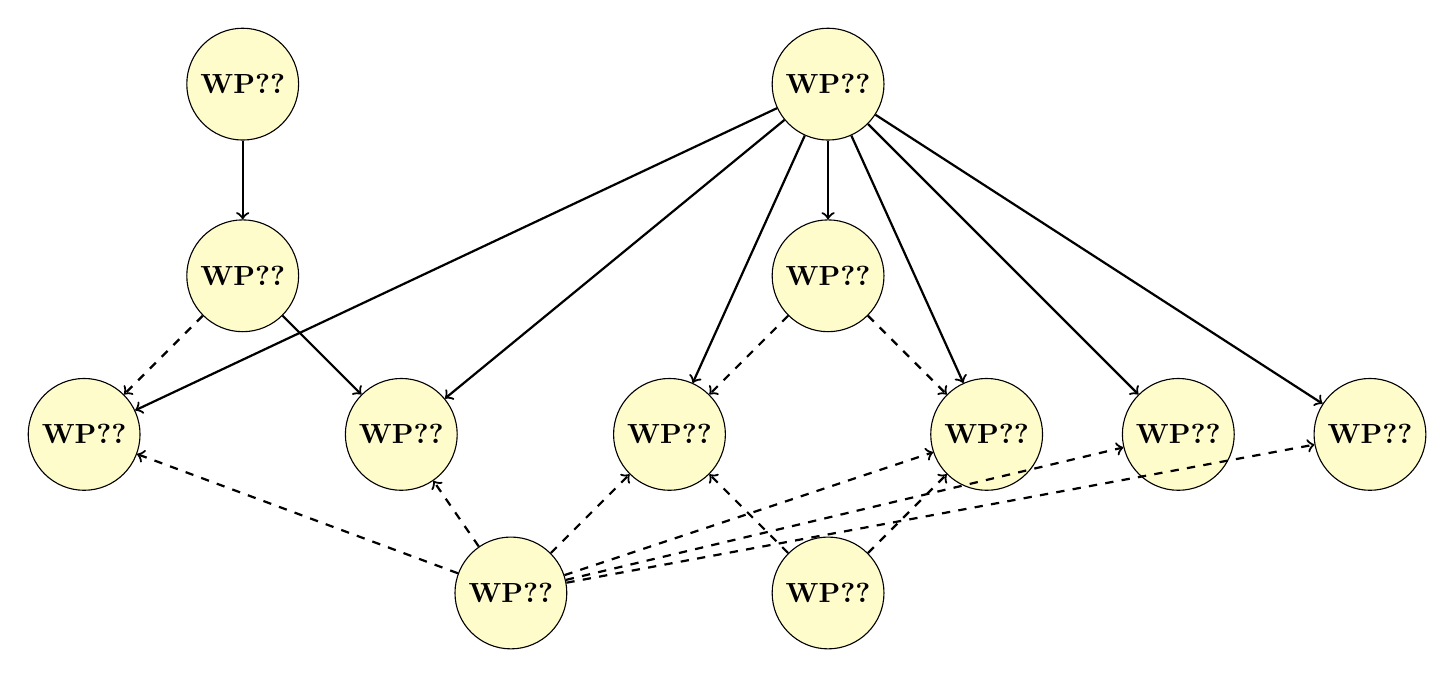
\begin{tikzpicture}
 \node[main node] (rei) {\WPref{wp:reimplement}} ;
\node[main node] (dom)[below=of rei] {\WPref{wp:domain}};
 \node[main node] (top)[below left = of dom] {\WPref{wp:topdown}};
 \node[main node] (unf)[below right = of dom] {\WPref{wp:unfounded}};
     \node[main node] (jus)[below right = of top] {\WPref{wp:just}};
    \node[main node] (lit)[left =6   of rei] {\WPref{wp:lit}};
            \node[main node] (fac)[below=of lit] {\WPref{wp:factors}};
                \node[main node] (qua)[below left=of fac] {\WPref{wp:quantify}};
    \node[main node] (app)[below left= of top] {\WPref{wp:application}};
        \node[main node] (alg)[below right=of fac] {\WPref{wp:algo:other}};

         \node[main node] (wat)[right=of unf] {\WPref{wp:watch}};

    \node[main node] (mag)[right=of wat] {\WPref{wp:magic}};
    \path[draw,thick,->]
        (lit)  edge node {} (fac);
    \path[draw,thick,->]
        (fac)  edge node {} (alg);
    \path[draw,thick,->]
        (rei)  edge node {} (alg);
    \path[draw,thick,dashed,->]
        (fac)  edge node {} (qua);   
    \path[draw,thick,->]
        (rei)  edge node {} (qua);   
    \path[draw,thick,->]
        (rei)  edge node {} (dom);   
    \path[draw,thick,->]
        (rei)  edge node {} (top);   
    \path[draw,thick,->]
        (rei)  edge node {} (unf);   
    \path[draw,thick,->]
        (rei)  edge node {} (mag);   
    \path[draw,thick,->]
        (rei)  edge node {} (wat);  
    \path[draw,thick,dashed,->]
        (dom)  edge node {} (top);   
    \path[draw,thick,dashed,->]
        (dom)  edge node {} (unf); 
    \path[draw,thick,dashed,->]
        (jus)  edge node {} (top);   
    \path[draw,thick,dashed,->]
        (jus)  edge node {} (unf); 
    \path[draw,thick,dashed,->]
        (app)  edge node {} (wat);   
    \path[draw,thick,dashed,->]
        (app)  edge node {} (mag);   
    \path[draw,thick,dashed,->]
        (app)  edge node {} (top);   
    \path[draw,thick,dashed,->]
        (app)  edge node {} (unf);  
    \path[draw,thick,dashed,->]
        (app)  edge node {} (qua);  
    \path[draw,thick,dashed,->]
        (app)  edge node {} (alg);  
    
% % 
% %     \node[main node] (1) {$1$};
% %     \node[main node] (2) [below left = 2.3cm and 1.5cm of 1]  {$2$};
% %     \node[main node] (3) [below right = 2.3cm and 1.5cm of 1] {$3$};
% 
%     \path[draw,thick]
%     (1) edge node {} (2)
%     (2) edge node {} (3)
%     (3) edge node {} (1);
%     %%
%     \begin{scope}[xshift=4cm]
% %     \node[main node] (1) {$1$};
% %     \node[main node] (2) [right = 2cm  of 1]  {$2$};
% %     \node[main node] (3) [below = 2cm  of 1] {$3$};
% %     \node[main node] (4) [right = 2cm  of 3] {$4$};
% 
%     \path[draw,thick]
%     (1) edge node {} (2)
%     (1) edge node {} (4)
%     (3) edge node {} (2)
%     (3) edge node {} (4)
%     ;
%     \end{scope}

\end{tikzpicture}
}
% \begin{tikzpicture}[node distance = {1.0cm and 1.5cm}, v/.style = {draw, circle}]
%   \graph[nodes={circle, draw}, grow right=2.25cm, branch down=1.75cm]{
%     A -- ["1"] C -- ["3"] E,
%     B -- ["1"] D -- ["4",swap] F,
%     B -- ["2"] A,
%     C -- ["2"] {D,B,G,H},
%     D -- ["3",swap] E -- ["1"] F,
%     G -- B
%   };
% \end{tikzpicture}
\caption{Dependencies between the different work packages.}
\label{fig:dependencies} 
\end{wrapfigure}

In case we experience set-backs, such as certain methods not working out in general, we will not hesitate to restrict our attention to a subset of all ASP programs for which we can get the techniques to work. 
Examples of such subsets include normal logic programs, $\omega$-restricted programs \cite{lpnmr/Syrjanen01}, $\lambda$-restricted programs \cite{lpnmr/GebserST07}, 
% which were the kind of programs accepted by lparse \cite{Syrjanen98} and the first versions of gringo \cite{lpnmr/GebserST07}  respectively, 
and generate-define-test programs \cite{Lifschitz/AI02}. 
These classes cover the majority of practical problems modeled in ASP, but impose syntactic restrictions that might enable techniques that do not work in general. 


% \todo{figure: dependencies of work packages}
% \label{wp:lit} \label{wp:factors}\label{wp:reimplement}\label{wp:quantify}\label{wp:improvements:first}\label{wp:topdown}\label{wp:unfounded}\label{wp:improvements:last}\label{wp:magic}\label{wp:application}\label{wp:algo:other}



% \todo{figure:



% \section{Analysis of risks and bottlenecks}
% Little to no risk is involved in the project as the commitment of the three groups  and their  expertise on
% the subject enables the attainability of the objectives. Cooperation between KRR and LIRIS  has already resulted in several joint publications \cite{ruleml/DassevilleJJVD16,caise/JanssensBSVD16} and a joint TETRA project ``Decision Analytics''.
% 
% The sustainability of the project is deemed high. We expect to maintain an active 
% relationship by submitting joint funding proposals, both between the participating groups and with external and
% international parties. This will lead to additional long-term benefits after the conclusion of the project
% and to the development of applications for use within practical domain areas.
% While dealing with companies to attain real-life cases may incur delays, this is expected not to be a
% problem since LIRIS has a lot of experience in this regard and we have a joint ongoing TETRA project with industry partners. Additionally, as indicated by the distribution of the
% work packages, the proposed research objectives can partly be tackled in parallel. This decreases the risk
% that delays in one objective may impact the outcome of others.
% 
% Since time is spent on algorithms and implementation, we will actively ensure that the project stays research-oriented and does not turn into an engineering project. 
% We only implement proof-of-concepts on top of the IDP system sufficient for experimentation, not a completely documented industry-proof system. 
% These ideas can later be implemented natively by the IDP development team. 

% \vspace{5mm}



% \subsection*{Budget, Added Value, and Leverage}
% 
% % % a brief but for the referees clearly reasoned budget estimate (the
% % \textbf{referees are asked to evaluate whether the budget applied for is
% % realistic for the proposed research; it is therefore important to
% % provide a clear motivation for the applied budget);}
% 
% % \todo{KERSTEN; Zullen de PhDs ook travel grants aanvragen (FWO, Doctoral Schools, Conference student coverage, …)?}
% 
% We apply for a 4 year project with 8MY for PhD students, i.e., 2 PhD students. 
% Additionally, we apply for \EUR{104.500} for consumables. The majority of this consumable budget consists of travel budget, to facilitate six-month stays of the students with our collaborators, the planned workshops and the additional short-term research visits. The rest of the consumables budget is to be used for funding conference visits to present our work, research material and equipment, open-access fees, and a share in a server or credits for running experiments on computer clusters. %: in total \EUR{80.000}. %When applicable, the PhD students will 
%  \item For each research visit per person: \EUR{500} (flights) + \EUR{500} per week or \EUR{1.650} per month, which is the standard FWO compensation for research visits. In total, this adds up to \EUR{49.800}. This includes the various workshops (including funds to invite two external researchers to each of them), two two-week research visits of Bogaerts, two six-month research visits of involved researchers, and four additional short-term (two week) incoming or outgoing research visits for two persons. 
%  \begin{compactitem}
%   \item For each of the workshops, 1 week for all persons involved in the project (who are not yet at the meeting location) and two extra (external) researchers: \EUR{18.000}. 
%   % 2+2  + 3+2   + 3+2    +   2+2 
%   \item Two additional two-week research visits of Bogaerts: \EUR{3.000}. 
%   \item One six-month stay of each PhD student: \EUR{20.800}. 
%   \item Four additional one-week research visits of two persons, as explained in Section \ref{sec:org}: \EUR{8.000}.
%  \end{compactitem}
% \end{compactitem}


% Given the breadth of the research, we do
% not expect we can realize all objectives with this manpower. However,
% as we did in the past for similar projects, we expect we can obtain
% extra manpower, either by attracting excellent students that can
% obtain an individual PhD grant or by submitting complementary projects
% to the Flemish Research Foundation (FWO).

% % a compactdesc of the scientific added value of the project and in
% general how the project will act as a leverage towards external
% funding (make sure to write this part in a way your external referees
% can understand).



% \section{Science Communication to Non-Experts}
% 
% Applications of answer set programming are very varied in nature and appeal to a wide audience of non-experts. 
% We plan to attract their attention by developing demos for science events such as ``Dag van de Wetenschap'' (the biggest science event in Flanders and Brussels). 
% Furthermore, we will, in collaboration with the ``wetenschaps expertise en communicatie cel'' (WECOM) of the VUB, regularly write blog posts (on \url{www.wtnschap.be}) and  press releases about applications of the developed tools; an example of such a press release on our latest paper on this topic can be found at \url{http://cs.aalto.fi/en/current/news/2018-07-18/}. 
% \end{document}

\newpage

{
\section*{References}
\scriptsize

% \linespread{2.1}\selectfont
\bibliographystyle{plain}
% \renewenvironment{thebibliography}[1]{%
% %   \section*{\refname}%
%   \let\par\relax\let\newblock\relax%
%   \inparaenum[{[}1{]}]}{\endinparaenum}
% \renewcommand{\bibitem}[1]{\item\label{#1}}
\bibliography{idp-latex/krrlib,more}
}

\end{document}
\todo{KERSTEN: DMP of data management plan, dit zal er zeker in zitten en is reeds een tab in de vorige call. Weet vooral dat VUB hier deels ondersteuning in kan/zal geven alsook via https://dmponline.be/ dat een aanzet geeft tot het adresseren van de nodige vragen.}

\todo{KERSTEN: Als niet-expert kan ik meegeven dat je voorstel heel technisch is geschreven (in mijn ogen). Ik vermoed dat naargelang de commissie of discipline waarin je zal indienen de experten deze techniciteit en jargon aankunnen? Wat ik als leek een beetje mis is om af en toe de overgangen in algemene taal te recapituleren en nadruk te leggen op het innovatieve en hoe alles aan elkaar hangt. Naar de experten toe kan het interessant zijn om heel duidelijk te zijn en op gepasten tijde je ‘core’-concept blijft herhalen.
}

\todo{verminder refs}


\todo{ KERSTEN: Indien je het volledige dossier hebt (met online ingevulde data ook) mag je dit gerust nog eens doorsturen. Als totaal non-expert in informatica zou ik vooral erop letten dat je voorstel logisch geordend is en het onderscheid tussen PhD 1 en 2 duidelijk is naar de experts die dit zullen lezen, ook dat deze beide studenten een compleet en (onafhankelijk) project kunnen uitvoeren wat FWO denk ik wel zal appreciëren.  }


\end{document}

\newpage
{
\color{red}

\section{Goals}
Two types of goals. 
The first focuses on justification theory. 
\begin{compactitem}
 \item Extend justification theory to capture disjunctive programs
\end{compactitem}

The second relates to programming techniques/algorithm. 
\begin{compactitem}
\item Extend a modern ASP solver (\wasp/clasp) with lazily grounded rules. Reasons:  
 \begin{compactenum}
  \item This allows us to quantify fairly how the performance of lazy grounding compares to the performance of modern solvers. 
  \item GOAL: identify weak points in current implementations of lazy grounding solvers that are NOT due to missing optimizations. 
  \begin{compactitem}
  \item Missing top-down propagation due to not knowing completion can be added. -> Quantify 
  \item Missing unfounded set propagation. 
  \item More propagation missing due to ungrounded rules? 
  \item Limited set of atoms to choose on: Only choices on whether body fires or not 
  \item 
  \end{compactitem}
  These things can be tested WITHOUT implementing lazy grounding. Is a good first step. 
 \end{compactenum}
 
 \item Develop techniques that compensate for the different types of missing propagation:
 \begin{compactitem}
 \item: completion: techniques for detecting htat all rules deriving a given atom are grounded: use domain estimation techniques from prolog/database theory? 
 \item: UFS: A dynamic version of the unfounded set algorithm that can work with non-completed atoms (atoms for which more rules might exist). 
 When one such atoms is propagated to be true, a call-back to the grounder  is made which triggers additional grounding
 \item For other propagation, develop a two-watched literal scheme that acts on non-ground rules. 
 \end{compactitem}
  

 \item A top-down lazy grounding algorithm with a cdcl back-end
%  \item 
 
\end{compactitem}
qdf

}



\end{document}
